\documentclass[english]{tktltiki}
\usepackage[pdftex]{graphicx}
\usepackage{subfigure}
\usepackage{url}
\usepackage{tabu}
\begin{document}
\onehalfspacing

\title{Assignment 5: Design Space Analysis}
\author{P�ter Ivanics}
\date{\today}

\maketitle

\numberofpagesinformation{\numberofpages\ pages + \numberofappendixpages\ appendices}
\keywords{}

\mytableofcontents

\section{Introduction}
	This report takes a look into design space analysis and levels of design variables through two case studies: a Baxter Colleague CX Infusion Pump (Figure \ref{baxter-pump}) and an Airbus A380 cockpit (Figure \ref{airbus-a380}). The report is rolled out as one of the assignment of the Human-Computer Interaction course and serves the purpose to gain hands-on experience with the course material. 
	
	To begin with, the two interfaces are described briefly and the design variables are chosen and introduced. Some hypothesis of the interfaces and the available controls are made. Further, an arguments are stated for the selected dimensions/variables and the size of the design space is calculated accordingly for both cases. Finally, the analysis is summarized.  
	
\section{Design Space Analysis}
	This section introduces the two interfaces and analyses their design space separately. First, the Baxter Infusion Pump, then the Airbus A380 cockpit is analyzed. 

	\subsection{Baxter Colleague CX Infusion Pump}
	The decision variables for such device correspond to the application field, the use case and the intended group of end-users of the device. In this case, I believe the infusion pump on Figure \ref{baxter-pump} is used mainly in clinical/medical settings mainly by nurses or doctors. The device is most probably used to deliver appropriate amount of desired medicine to the patient's body and therefore has a high responsibility. A potential malfunction and misuse of the device may lead to serious consequences. Also it is worth noticing that the device is an "expert system" and used by specialists, probably only in certain scenarios. 
	
	Accordingly, one could consider guidelines as an important decision variable in this case. In this setting this is demonstrated for instance by placing the three steps of how to load the device properly before usage (annotated with light green). As these instructions are placed in a clearly visible place it is ensured, that users of this device will know how to perform the installation of the device properly. On top of that, the handlebar on the right side of the device has a label of "push" which further helps assisting the user how to use the device. I am not sure what the handlebar is for, however I guess it is something which should be pushed down to lock it into place while operating. 
	
	A second aspect would be informativeness and feedback the displays. The two displays in the left side of the screen (highlighted with red) are probably monitoring the patient's current health and need for the required medication. As the space is limited, a designer should consider how much space is dedicated to what type of information in such situation. Furthermore, the device may have speakers to play auditory information, however this dimension is excluded from the analysis.
	
	The three led lights between the two screens (purple) are somewhat similar, however designers had chance to forward information with colors in this case. Notice that the middle led (with the label pumping) has a green color while the others on the side (alarm and alert) are red. The distinct color of these lights surely indicate the importance of the situation when they are lighted up (e.g. the green light gives feedback of correctness, while the red light probably requires some attention in unexpected situations). Consequently, usage of colors and indicators is an important decision variable in the design in this setting. The usage of colors also matters for the other buttons used for interaction and giving input to the device. Notice the five different color of buttons (black, green, red, white and orange).
	
	Last, but not least the device requires some input and interaction. Accordingly, there are plenty of buttons on the device (annotated with blue color), including a numerical pad, a button turning on the back light, changing the information on the screens and so on. The buttons on the device consistently follow the same design: they are slightly rounded and clearly visible, only their color differs in certain cases. As there are buttons which have on and off state, I would guess that these have two possible values indicating the on status with background color. Upon designing the device the designer surely had to consider other options, such as switches, sliders or other solutions. 
	
	\begin{figure}[h] 
		\begin{center}
			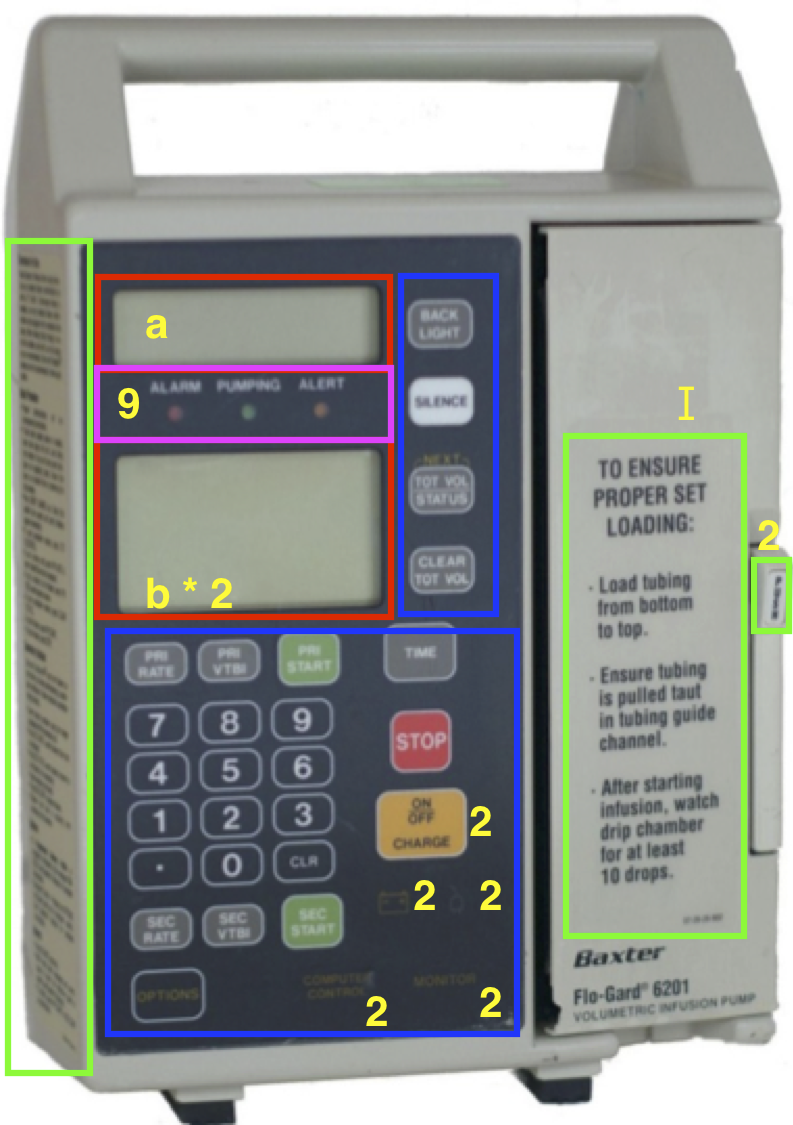
\includegraphics[width=0.6\textwidth]{images/Baxter-Colleague-CX-Infusion-Pump.png}
			\caption{Design A: a Baxter Colleague CX Infusion Pump.}
			\label{baxter-pump}
		\end{center}
	\end{figure}	
	
	To sum up, the prioritized dimensions are, as follows:
	\begin{enumerate}
		\item informativeness/feedback,
		\item colors,
		\item input controls (buttons, switches, sliders or other controls),
		\item guidelines.
	\end{enumerate}

	In order to calculate the size of the design space, the following assumptions are made: 
	\begin{itemize}
		\item the instructions take $I$ of the design space,
		\item the lever on the right side of the device (with the "Push" label) has two settings:
		\begin{itemize}
			\item normal status (as shown on the picture),
			\item fixed (pushed down).
		\end{itemize}
		\item the upper screen displays one line of information,
		\item the lower screen displays two lines of information,
		\item the led lights between the screens can have three statues:
			\begin{itemize}
				\item blank (not lighted up),
				\item lighted up,
				\item flashing.
			\end{itemize}
		\item the orange button (below "Stop") and the four small indicators below it have two statuses:
			\begin{itemize}
				\item on,
				\item off.
			\end{itemize}
		\item there are 25 buttons in total, which have only a single status (e.g. the numbers on the numerical pad).
	\end{itemize}
	
	Accordingly, the yellow numbers on Figure \ref{baxter-pump} indicate the values of the variables. The buttons which are assumed to have only one possible value are not annotated, but included in the calculation. The design space is calculated, as follows:
	
	\begin{eqnarray*}
		S = I + a + b * 2 + 9 + 6 * 2 + 25 = I + a + 2b + 46
	\end{eqnarray*}
	
	\subsection{Airbus A380 cockpit}
	Similarly to the previous case, the setting in which the Airbus A380 cockpit (Figure \ref{airbus-a380}) is used is important to define. This is a very special and complicated interface as the application ares is very specific, it is operated by two experts who are driving the airplane. Accordingly, there are plenty of controls, screens, colors as well as types of controls at the first glance. Certainly, the users of the system learn and train on this or similar cockpits in advance of using in a real setting. 
	
	Keeping the prior training in mind, it is expected that the pilots know how to operate with the plane's controls in general. The first aspect coming to my mind when looking at the cockpit is the wide variety and the huge number of controls. There is at least two type of "joystick" (annotated with red and green), which are probably responsible for coordinating the plane and adjusting its speed and altitude. In addition to that, a lot of different possibilities of adjustments are observed (highlighted with light blue color), for instance there are complete keyboards, sliders, switches, rotate-able controls and many others.
	
	Plenty of variables are responsible for showing visual response to the pilots (annotated with purple). Some of these potentially display external view through cameras attached to the body of the plane, provide weather and wind information, altitude, speed, engine health and other measures. The displayed colors in the screens play a huge role as they forward a lot of information to the pilot, for example warning them about a storm ahead or strong wind from certain direction. 
	
	I assume that these variables only display animations and are not taking any input through touchscreen. Typically there are microphones and speakers/headsets to communicate with the crew and the control towers/airports (I could not identify these on the photo). 
	
	\begin{figure}[h] 
		\begin{center}
			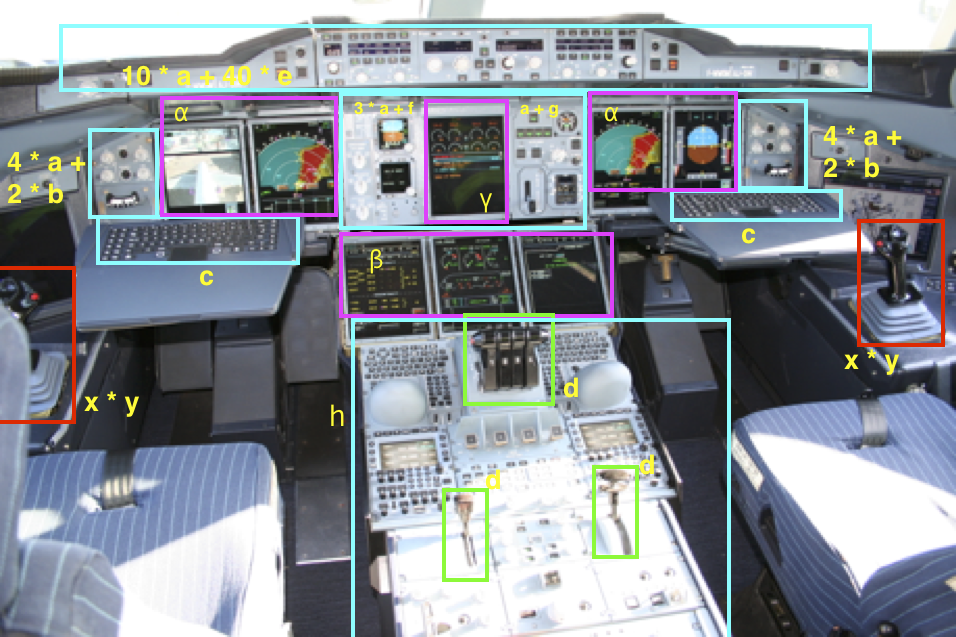
\includegraphics[width=0.8\textwidth]{images/Airbus-A380-cockpit.png}
			\caption{Design B: the cockpit of an Airbus A380.}
			\label{airbus-a380}
		\end{center}
	\end{figure}	
	
	From a designer point of view this is a real challenge. Keeping the design simple is impossible for outsiders, however pilots surely know how to operate such system. The most important variables in this case could be as follows:
	
	\begin{enumerate}
		\item positioning the controls: important to notice that both pilots have access to more or less the same controls and therefore most of them are duplicated. This can be explained by the fact that the airplane is demanding to drive and one can simply not divide their attention enough. On top of that, the space is limited and both pilots have to have arm-distance access to all of these controls. 
		\item communication: as pilots have to communicate with multiple parties and eachother, the interface should facilitate the fluent flow of communcation as much as possible. 
		\item feedback and monitoring: undoubtedly as a pilot keeping track of the plane's health is essential. For this reason, the screens which provide feedback about the status of components and external factors (e.g. weather) are crucial and have to be designed carefully. This means the screen size, resolution, proper selection of colors as well as positioning these items on the dashboard correctly. 
		\item informativeness: on top of how feedback is provided and how screens are positioned, the displayed information has to be informative. For instance, displaying the weather on a radar and the height and speed as numbers are seem to be appropriate choices. The designer of such aircraft had to deeply understand the possibilities as well as the opinion of pilots, how data from sensors can be represented efficiently. 
		\item possible states and complexity of the input controls: is the switch only on or off, how many states a rotate-able control can have, on which axis a joystick is moving (only one direction or two directions, for instance the ones highlighted with red move on two axis, while the green ones only move only on one axis). 
	\end{enumerate}
	
	In order to calculate the size of the design space, the following assumptions are made: 
	\begin{itemize}
		\item the left side of the cockpit is identical to the right side (as both pilots have access to the same controls),
		\item the joysticks highlighted with red move in a two-dimensional space (up, down, left, right) - donated with $x * y$,
		\item the joysticks highlighted with green move in a one-dimensional space (forward, backward) - donated with $d$,
		\item there are two type of rotate-able controls over the dashboard (e.g. on the left side of the photo, just above the keyboard),
		\begin{enumerate}
			\item white, donated with $a$,
			\item black, donated with $b$,
		\end{enumerate}
		\item keyboards have $c$ number of buttons,
		\item in the top dashboard (below the windshield) there are 10 of type $a$ switches and 40 buttons,
		\item the space which is between the two seats has $h$ buttons,
		\item the space between the output devices donated with $\alpha$, $\beta$ and $\gamma$ have $f$ and $g$ buttons,
		\item output devices (annotated with purple and their design spaced donated with Greek letters) have complex design space and should be analyzed separately,
		\item the design space of the headsets and microphones, which is used by both pilots is donated by $H$ and should be analyzed separately. 
	\end{itemize}
	
	Accordingly, the design space is approximated, as follows: 
	\begin{eqnarray*}
		S = 2 * (x * y + 4 * a + 2 * b + \alpha + H) + 3 * a + f + a + g + \beta + \gamma + 3 * d + h
	\end{eqnarray*}

\section{Conclusions}
	To sum up, we can easily see that the Airbus cockpit (Figure \ref{airbus-a380}) has a much bigger design space in comparison to the infusion pump (Figure \ref{baxter-pump}). Despite the fact that they share some similarities, the former uses a wider selection of variables, input and output controls and therefore yields in a more complex design space. 
\nocite{*}
\bibliographystyle{tktl}
\bibliography{bibliography}

\lastpage

\end{document}